% !TeX program = xelatex
% !TeX encoding = UTF-8
% 编译两次：xelatex ism-paper.tex
\RequirePackage{iftex}
\ifPDFTeX
  \PassOptionsToClass{fontset=windows}{ctexart}
\else
  \PassOptionsToClass{fontset=fandol}{ctexart}
\fi
\documentclass[UTF8,a4paper,zihao=-4]{ctexart}
\usepackage[top=23mm,bottom=23mm,left=24mm,right=24mm]{geometry}
\usepackage{amsmath,amssymb,booktabs,tabularx,array}
\usepackage{enumitem,float,needspace}
\usepackage{listings,setspace}
\usepackage{graphicx,tikz}
\usetikzlibrary{arrows.meta}
\usepackage[font=small,labelfont=bf,labelsep=quad,skip=5pt]{caption}
\usepackage{pdfpages}
\usepackage[hidelinks]{hyperref}

\hypersetup{
  pdftitle={大学生就业焦虑驱动因素分析},
  pdfauthor={刘佳辉},
  pdfsubject={基于 ISM 模型的五级递阶解释}
}
\ctexset{
  section={format=\Large\bfseries,name={,},number=\arabic{section},aftername=\quad,
    beforeskip=14pt,afterskip=6pt},
  subsection={format=\normalsize\bfseries,aftername=\quad,beforeskip=9pt,afterskip=4pt}
}
\onehalfspacing
\raggedbottom
\pagestyle{plain}
\clubpenalty=10000
\widowpenalty=10000
\renewcommand{\arraystretch}{1.16}
\newcolumntype{L}[1]{>{\raggedright\arraybackslash}p{#1}}
\newcolumntype{Y}{>{\raggedright\arraybackslash}X}
\setlist[enumerate]{topsep=3pt,itemsep=2pt,parsep=0pt}
\setlength{\intextsep}{8pt plus 2pt minus 2pt}
\captionsetup[table]{position=top}
\newcommand{\factor}[1]{\ensuremath{S_{#1}}}
\newcommand{\lev}[1]{\ensuremath{L_{#1}}}

% 黑白灰配色与共用的 TikZ 样式。
\definecolor{ismLight}{gray}{0.91}
\definecolor{ismText}{gray}{0.24}
\definecolor{ismGrid}{gray}{0.48}
\definecolor{ismZero}{gray}{0.35}
\definecolor{ismRule}{gray}{0.67}
\tikzset{
  ism canvas/.style={x=1mm,y=-1mm,font=\sffamily},
  ism title/.style={font=\sffamily\bfseries\large,text=black,inner sep=0pt},
  ism note/.style={font=\sffamily\small,text=ismText,inner sep=0pt},
  ism cell note/.style={font=\sffamily\footnotesize,text=ismText,inner sep=0pt},
  ism edge/.style={draw=black,line width=.75pt,-{Triangle[length=2.1mm,width=1.8mm]}},
  ism skip edge/.style={ism edge,draw=black,dash pattern=on 3pt off 1.7pt},
  ism circle/.style={circle,fill=white,draw=black,line width=.65pt,
    minimum size=8mm,inner sep=0pt,text=black,font=\sffamily\bfseries\normalsize},
  ism band/.style={font=\sffamily\bfseries\footnotesize,
    anchor=west,inner sep=0pt,text=ismText},
  ism box/.style={draw=black,line width=.7pt,
    minimum height=9mm,inner sep=2pt,fill=white,text=black,
    font=\sffamily\bfseries\footnotesize,align=center}
}
\newcommand{\ismBounds}[2]{\path[use as bounding box] (0,0) rectangle (#1,#2);}
\newcommand{\ismFigure}[3]{%
  \begin{figure}[H]
    \centering
    #3\par
    \caption{#2}\label{fig:#1}
  \end{figure}%
}

% 图 1：分析流程。
\newcommand{\ismFlow}{%
  \begin{tikzpicture}[ism canvas]
    \ismBounds{158}{49}
    \node[ism title] at (81,7.8) {大学生就业焦虑驱动因素的 ISM 分析流程};
    \foreach \i/\heading/\detail in {
      0/明确问题/界定就业焦虑,
      1/识别因素/形成 S1—S8,
      2/判断关系/建立邻接矩阵 A,
      3/计算闭包/得到可达矩阵 M,
      4/重排矩阵/方框划分层级,
      5/绘制模型/梳理驱动路径,
      6/解释结果/提出分层建议
    }{
      \pgfmathsetmacro{\x}{25.5+18.65*\i}
      \ifnum\i<6
        \draw[black,line width=.55pt,-{Triangle[length=1.15mm]}]
          (\x+8.3,25.5) -- (\x+10.05,25.5);
      \fi
      \path[fill=white,draw=black,line width=.57pt]
        (\x-8.3,16.9) rectangle (\x+8.3,34.2);
      \node[font=\sffamily\bfseries\footnotesize,text=black,inner sep=0pt]
        at (\x,23.85) {\heading};
      \node[font=\sffamily\fontsize{6.3}{7.4}\selectfont,
        text=ismText,inner sep=0pt] at (\x,29.4) {\detail};
    }
    \node[ism cell note] at (82.4,40)
      {因素识别 \(\to\) 关系建模 \(\to\) 层级解释 \(\to\) 对策转化};
  \end{tikzpicture}%
}

% 图 2 与图 7 共享直接关系图，后者加上层级标识。
\newcommand{\ismNodeGraph}[3]{%
  \begin{tikzpicture}[ism canvas]
    \ismBounds{124}{#2}
    \node[ism title] at (62,4.6) {#1};
    \ifnum#2=95
      \foreach \y/\n/\role in {
        10/1/结果层,26/2/直接驱动层,42/3/传导层,
        58.5/4/基础驱动层,75.5/5/根源层
      }{
        \draw[ismRule,line width=.4pt]
          (8,\y+13.1) -- (116,\y+13.1);
        \node[ism band] at (3,\y) {L\n\enskip\role};
      }
    \fi
    \foreach \factor/\x/\y in {
      8/62/15.7,4/62/31.7,3/26.5/47.9,5/62/47.9,
      7/97.5/47.9,1/26.5/65,2/97.5/65,6/26.5/82.1
    }{
      \node[ism circle] (f\factor) at (\x,\y) {S\factor};
    }
    \foreach \from/\target in {1/3,2/5,2/7,3/4,4/8,5/4,6/1,7/4}{
      \draw[ism edge,shorten <=1pt,shorten >=1.3pt] (f\from) -- (f\target);
    }
    \draw[ism skip edge,shorten <=.5pt,shorten >=1.2pt]
      (f1.60) .. controls (36,50) and (47,42) .. (f4.240);
    \node[ism note] at (62,#2-3.3) {#3};
  \end{tikzpicture}%
}

% 图 3–6 共用矩阵数据。每行依次对应 S1 至 S8，每行内列顺序相同。
\ExplSyntaxOn
\newcommand{\ismMatrixRow}[3]{\cs_new:cpn { ism#1row#2 } {#3}}
\newcommand{\ismMatrixCell}[3]{\exp_args:Nv \str_item:nn { ism#1row#2 } {#3}}
\ExplSyntaxOff
\ismMatrixRow{A}{1}{00110000}
\ismMatrixRow{A}{2}{00001010}
\ismMatrixRow{A}{3}{00010000}
\ismMatrixRow{A}{4}{00000001}
\ismMatrixRow{A}{5}{00010000}
\ismMatrixRow{A}{6}{10000000}
\ismMatrixRow{A}{7}{00010000}
\ismMatrixRow{A}{8}{00000000}
\ismMatrixRow{M}{1}{10110001}
\ismMatrixRow{M}{2}{01011011}
\ismMatrixRow{M}{3}{00110001}
\ismMatrixRow{M}{4}{00010001}
\ismMatrixRow{M}{5}{00011001}
\ismMatrixRow{M}{6}{10110101}
\ismMatrixRow{M}{7}{00010011}
\ismMatrixRow{M}{8}{00000001}
% 参数：矩阵、标题、图内说明、行列顺序、是否描绘层级方框。
\newcommand{\ismMatrix}[5]{%
  \begin{tikzpicture}[ism canvas,x=8.9mm,y=-8.9mm]
    \ifx#1A
      \ismBounds{9.3}{10.55}
      \node[ism title] at (5.2,.43) {#2};
    \else
      \ismBounds{11.25}{10.55}
      \node[ism title] at (5.2,.43) {#2};
      \node[ism cell note] at (10.2,1.48) {行内“1”数};
    \fi
    \node[ism cell note] at (5.2,1.0) {#3};
    \node[ism cell note,rotate=90] at (.25,5.73) {行：影响因素};
    \node[ism cell note] at (5.15,10.21) {列：被影响因素};
    \fill[white] (1.15,1.85) rectangle (9.15,9.85);
    \foreach \r [count=\ri from 0] in {#4}{
      \node[font=\sffamily\bfseries\small,text=black,inner sep=0pt]
        at (.82,\ri+2.35) {S\r};
      \node[font=\sffamily\bfseries\small,text=black,inner sep=0pt]
        at (\ri+1.65,1.48) {S\r};
      \ifx#1M
        \node[font=\sffamily\bfseries\small,text=black,inner sep=0pt]
          at (10.2,\ri+2.35) {\inteval{%
            \ismMatrixCell{#1}{\r}{1}+\ismMatrixCell{#1}{\r}{2}+
            \ismMatrixCell{#1}{\r}{3}+\ismMatrixCell{#1}{\r}{4}+
            \ismMatrixCell{#1}{\r}{5}+\ismMatrixCell{#1}{\r}{6}+
            \ismMatrixCell{#1}{\r}{7}+\ismMatrixCell{#1}{\r}{8}}};
      \fi
      \foreach \c [count=\ci from 0] in {#4}{
        \edef\cellvalue{\ismMatrixCell{#1}{\r}{\c}}
        \ifnum\cellvalue=1
          \fill[ismLight] (\ci+1.15,\ri+1.85) rectangle ++(1,1);
          \node[font=\sffamily\bfseries,text=black,inner sep=0pt]
            at (\ci+1.65,\ri+2.35) {1};
        \else
          \node[font=\sffamily,text=ismZero,inner sep=0pt]
            at (\ci+1.65,\ri+2.35) {0};
        \fi
      }
    }
    \foreach \i in {0,...,8}{
      \draw[ismGrid,line width=.32pt] (\i+1.15,1.85) -- (\i+1.15,9.85);
      \draw[ismGrid,line width=.32pt] (1.15,\i+1.85) -- (9.15,\i+1.85);
    }
    \ifnum#5=1
      \foreach \start/\blocksize/\level in {0/1/1,1/1/2,2/3/3,5/2/4,7/1/5}{
        \draw[black,line width=1.25pt]
          (\start+1.15,\start+1.85) rectangle ++(\blocksize,\blocksize);
        \node[anchor=north west,fill=white,
          text=black,font=\sffamily\bfseries\scriptsize,inner sep=.5pt]
          at (\start+1.27,\start+1.95) {L\level};
      }
    \fi
  \end{tikzpicture}%
}

% 图 8：完整因素名称与五级带状布局。
\newcommand{\ismNamedGraph}{%
  \begin{tikzpicture}[ism canvas]
    \ismBounds{142}{100.5}
    \node[ism title] at (71,4.2) {大学生就业焦虑驱动因素解释结构模型};
    \foreach \y/\n/\role in {
      8.1/1/结果层,24.6/2/直接驱动层,41.9/3/传导层,
      59.8/4/基础驱动层,78.4/5/根源层
    }{
      \draw[ismRule,line width=.4pt]
        (4,\y+13.4) -- (138,\y+13.4);
      \node[ism band] at (3.5,\y) {L\n\enskip\role};
    }
    \node[ism box,minimum width=35mm,fill=black!75,text=white]
      (f8) at (72,14) {S8\enskip 就业焦虑};
    \node[ism box,minimum width=45mm,fill=ismLight]
      (f4) at (72,30.5) {S4\enskip 害怕面试失败或被拒绝};
    \node[ism box,minimum width=35mm]
      (f3) at (29,48.6) {S3\enskip 自身专业技能不足};
    \node[ism box,minimum width=35mm]
      (f5) at (67,48.6) {S5\enskip 同辈比较与内卷压力};
    \node[ism box,minimum width=39mm]
      (f7) at (106.8,48.6) {S7\enskip 招聘信息获取渠道不畅};
    \node[ism box,minimum width=35mm]
      (f1) at (29,67) {S1\enskip 缺乏清晰的职业规划};
    \node[ism box,minimum width=39mm]
      (f2) at (106.8,67) {S2\enskip 就业市场竞争激烈};
    \node[ism box,minimum width=39mm]
      (f6) at (31,85.1) {S6\enskip 家庭期望与经济压力};
    \draw[ism edge,shorten <=2pt,shorten >=2pt] (f6.north) -- (f1.south);
    \draw[ism edge,shorten <=2pt,shorten >=2pt] (f1.north) -- (f3.south);
    \draw[ism edge,shorten <=2pt,shorten >=2pt] (f2.north) -- (f7.south);
    \draw[ism edge,shorten <=.6pt,shorten >=1.1pt] (97,62.5) -- (75,53.1);
    \draw[ism edge,shorten <=.6pt,shorten >=1.1pt] (37,44.1) -- (57,35);
    \draw[ism edge,shorten <=2pt,shorten >=2pt] (f5.north) -- (70,35);
    \draw[ism edge,shorten <=.6pt,shorten >=1.1pt] (100,44.1) -- (81,35);
    \draw[ism edge,shorten <=2pt,shorten >=2pt] (f4.north) -- (f8.south);
    \draw[ism skip edge,shorten <=1pt,shorten >=1.3pt]
      (42,62.5) .. controls (47,56) and (46.8,49) .. (48,44.2)
                .. controls (49.2,40.5) and (58,37.8) .. (63.5,35);
    \node[ism note] at (71,96.5)
      {深层根源通过职业规划、能力/信息与市场比较等路径向上传导，最终表现为就业焦虑};
  \end{tikzpicture}%
}

\begin{document}

\hypersetup{pageanchor=false}

\includepdf[pages=1,fitpaper=true,pagecommand={\thispagestyle{empty}}]{cover.pdf}
\setcounter{page}{1}
\hypersetup{pageanchor=true}

\noindent\makebox[\linewidth][c]{\bfseries\abstractname}\par
\nobreak\smallskip
本文以大学生秋招与春招为研究情境，运用解释结构模型（ISM）梳理就业焦虑的驱动因素及作用路径。依据研究者对八个因素之间九条直接影响关系的判断，构建邻接矩阵，计算布尔闭包，并用可达集与先行集逐层划分。结果得到由结果层、直接驱动层、传导层、基础驱动层和根源层构成的五级结构。害怕面试失败或被拒绝直接触发就业焦虑；技能不足、同辈比较和信息不畅经此节点传导；家庭期望与经济压力经职业规划影响能力准备和面试预期。本文据此从个体、学校、家庭及环境与政策层面提出建议。

\noindent\textbf{关键词}\quad 大学生就业焦虑；解释结构模型；驱动因素；层级划分

\section{问题界定与研究设计}

\subsection{研究背景与核心问题}

秋招与春招期间，大学生需要在较短时间里完成自我定位、信息筛选、简历投递、笔试面试和多方比较。就业结果的不确定性，加上同辈进度、家庭期待和沉没成本，容易使焦虑从暂时性的情绪反应演变为持续的回避行为。若只把焦虑理解为“心态不好”，就会忽略它背后的结构性成因；若只归因于就业市场，又难以解释为什么处在相似环境中的学生会出现明显不同的焦虑水平。

因此，本报告要回答的核心问题不是“焦虑有多严重”，而是：哪些因素把大学生推向就业焦虑，这些因素通过怎样的路径发生作用，哪些是表层触发，哪些是深层根源？对该问题的回答，可以为个体调适、学校就业服务和家庭沟通提供更有针对性的切入点。

\subsection{方法选择与分析路线}

就业焦虑的驱动因素之间并非并列关系。职业规划会影响技能准备，技能准备又会改变面试信心；家庭压力可能先影响规划，再经由能力和面试环节传导；同辈比较与信息差则会放大失败预期。面对这种“因素多、关系杂、层级不清”的问题，解释结构模型（Interpretive Structural Modeling，ISM）具有较好的适配性：它不要求大样本测量，而是把专家或研究者的关系判断转化为邻接矩阵与可达矩阵，再通过层级划分把复杂系统还原为可解释的递阶结构。

本报告的分析路线如图~\ref{fig:flow} 所示：先界定问题与因素集合，再判断因素间的直接影响关系，随后计算可达矩阵、重排矩阵并完成层级划分，最后把数学结果转译为解释结构模型和对策建议。

\ismFigure{flow}{大学生就业焦虑驱动因素的 ISM 分析流程}{%
  \ismFlow%
}

\subsection{研究边界与基本假设}

第一，本报告分析的是因素之间的结构关系，不测量各因素的权重或焦虑得分，因此结论用于解释作用路径，不用于判断某一因素的统计效应大小。第二，因素集合来自秋招、春招情境下的典型表现与小组讨论，选取的是具有代表性且可操作的八个因素，并未穷尽所有个体差异。第三，因素间的直接关系由研究者依据情境逻辑作出判断。ISM 的输出质量取决于关系判断的质量，因此后文会明确每条关系的理由，并在结论部分说明模型边界。

\subsection{符号与矩阵规则}

记因素集合为 \(S=\{S_1,S_2,\ldots,S_8\}\)，有序对 \((S_i,S_j)\) 表示 \(S_i\) 对 \(S_j\) 存在直接影响。邻接矩阵 \(A=(a_{ij})\) 中，若存在该直接影响，则 \(a_{ij}=1\)，否则为 \(0\)；行表示影响来源，列表示影响去向。可达矩阵 \(M\) 在邻接矩阵基础上加入单位矩阵并求布尔闭包，既保留直接影响，也保留经过一条或多条路径形成的间接影响。

\section{要素识别与关系判断}

\subsection{八个驱动因素的界定}

为避免“就业焦虑”成为一个笼统标签，本报告把驱动因素划分为个体认知与能力、就业环境、同伴比较、家庭支持和信息披露五类，并统一编码为 \factor{1}—\factor{8}，如表~\ref{tab:factors} 所示。\factor{8} 是结果变量，其余七个因素为解释变量。

\begin{table}[H]
  \centering
  \small
  \caption{大学生就业焦虑驱动因素体系}\label{tab:factors}
  \begin{tabularx}{\linewidth}{@{}cL{43mm}Yc@{}}
    \toprule
    编号 & 驱动因素 & 具体含义 & 系统角色 \\
    \midrule
    \factor{1} & 缺乏清晰的职业规划 & 对职业方向、行业选择和求职节奏缺少明确安排，行动依赖临时反应 & 基础驱动 \\
    \factor{2} & 就业市场竞争激烈 & 岗位供给、招聘门槛、竞争者数量共同造成的外部压力 & 环境基础 \\
    \factor{3} & 自身专业技能不足 & 专业知识、实习经历、项目能力和简历表达未形成竞争力 & 能力传导 \\
    \factor{4} & 害怕面试失败或被拒绝 & 对面试评价、拒绝结果和失败后果的担忧，伴随回避倾向 & 直接触发 \\
    \factor{5} & 同辈比较与内卷压力 & 以同学 Offer、进度和选择为参照形成的相对落后感 & 比较传导 \\
    \factor{6} & 家庭期望与经济压力 & 家庭对稳定、回报和时间节点的期待，以及经济支持的不确定性 & 深层根源 \\
    \factor{7} & 招聘信息获取渠道不畅 & 招聘信息分散、时效性差、理解成本高，形成信息差 & 信息传导 \\
    \factor{8} & 就业焦虑 & 面对求职不确定性产生的紧张、担忧和回避等综合反应 & 结果变量 \\
    \bottomrule
  \end{tabularx}
\end{table}

这八个因素并不是简单并列。\factor{8} 是系统的输出端；\factor{4} 位于输出端之前，是最接近焦虑的体验性因素；\factor{3}、\factor{5}、\factor{7} 分别从能力、比较和信息三个方向把压力推向 \factor{4}；\factor{1}、\factor{2} 提供更基础的行动条件与环境条件；\factor{6} 则通过家庭情境影响个体的规划与选择。后续矩阵计算将检验这一直觉判断是否成立。

\Needspace{38mm}
\subsection{直接关系集合}

依据“前者是否会在现实求职过程中直接推动后者”的判断标准，共识别出 9 条直接关系。关系集合见式~\eqref{eq:relations}，各条关系的判断依据见表~\ref{tab:relations}。

\begin{equation}
  \begin{aligned}
    R = \{& (S_1,S_3),(S_1,S_4),(S_2,S_5),(S_2,S_7),(S_3,S_4),\\
          & (S_4,S_8),(S_5,S_4),(S_6,S_1),(S_7,S_4) \}.
  \end{aligned}
  \label{eq:relations}
\end{equation}

\begin{table}[H]
  \centering
  \small
  \caption{因素间的直接关系及解释}\label{tab:relations}
  \begin{tabularx}{\linewidth}{@{}ccY@{}}
    \toprule
    序号 & 直接关系 & 关系解释 \\
    \midrule
    1 & \(S_{1}\to S_{3}\) & 缺少规划会减少针对性学习、实习和项目积累，导致技能准备不足 \\
    2 & \(S_{1}\to S_{4}\) & 方向不清会直接增加面试中的不确定感，形成对失败的预期 \\
    3 & \(S_{2}\to S_{5}\) & 竞争越激烈，个体越容易以同辈进度作为自我评价参照 \\
    4 & \(S_{2}\to S_{7}\) & 岗位要求提高、信息更新加快，会放大信息获取与理解难度 \\
    5 & \(S_{3}\to S_{4}\) & 能力与经历不足会降低面试信心，提高失败预期 \\
    6 & \(S_{4}\to S_{8}\) & 对失败和拒绝的担忧是最接近焦虑体验的直接触发 \\
    7 & \(S_{5}\to S_{4}\) & 同辈比较把“别人已经拿到”转化为“自己可能失败”的压力 \\
    8 & \(S_{6}\to S_{1}\) & 家庭期待与经济压力会影响职业选择的时间表和风险偏好 \\
    9 & \(S_{7}\to S_{4}\) & 信息差导致准备失焦、错投漏投，进而增加面试失败风险 \\
    \bottomrule
  \end{tabularx}
\end{table}

\subsection{直接关系图}

将上述关系绘制为有向图（图~\ref{fig:direct}），可以直观看到关系的汇聚与分叉：\factor{4} 汇聚了 \factor{1}、\factor{3}、\factor{5}、\factor{7} 四条直接路径，\factor{1} 则承接 \factor{6} 并分叉到 \factor{3} 与 \factor{4}。图中用虚线标出 \(S_{1}\to S_{4}\) 的跨层直接关系：它说明职业规划不仅通过能力准备间接影响面试信心，也会直接改变个体对不确定性的解释。

\ismFigure{direct}{就业焦虑驱动因素的直接关系图}{%
  \ismNodeGraph{就业焦虑驱动因素的直接关系图}{94}
  {箭头表示直接影响，虚线表示跨层直接关系 \(S_1\!\to\!S_4\)}%
}

需要强调的是，图中箭头表示“直接影响”，不表示影响强度。比如 \(S_{2}\to S_{5}\) 与 \(S_{6}\to S_{1}\) 都只有一条箭头，但二者作用的现实时间尺度并不相同：前者可能随招聘季迅速放大，后者则更深地嵌入家庭决策与成长经历。ISM 解决的是路径和层级问题，强度问题需要后续测量研究补充。

\section{ISM 模型计算}

\subsection{建立邻接矩阵 A}

按照“行是起点、列是终点”的规则，把 9 条直接关系写入 \(8\times8\) 邻接矩阵（见图~\ref{fig:adjacency}）。若 \(S_i\) 直接影响 \(S_j\)，对应位置记为 1；否则记为 0。矩阵中每行“1”的数量反映该因素向外发出的直接关系数，每列“1”的数量反映其受到的直接推动数量。

\ismFigure{adjacency}{邻接矩阵 A}{%
  \ismMatrix{A}{邻接矩阵 A}
  {依据 9 条直接关系建立；行代表起点，列代表终点}{1,2,3,4,5,6,7,8}{0}%
}

邻接矩阵只记录一步关系，尚不能回答“\factor{6} 是否会经过 \factor{1}、\factor{3} 最终影响 \factor{8}”这类问题。要得到完整的传导路径，需要继续计算可达矩阵。

\subsection{计算可达矩阵 M}

在邻接矩阵上加入单位矩阵 \(I\)，得到 \(A+I\)，再通过布尔乘法不断迭代，直到矩阵不再变化：

\begin{equation}
  M=(A+I)^k,\qquad (A+I)^k=(A+I)^{k+1}.
  \label{eq:closure}
\end{equation}

计算得到的可达矩阵如图~\ref{fig:reachability} 所示。矩阵中的 1 表示行因素能够沿某条路径到达列因素，对角线上的 1 表示因素可达自身。与邻接矩阵相比，\(M\) 新增了间接路径，例如 \factor{6} 对 \factor{4}、\factor{8} 的可达关系，以及 \factor{2} 对 \factor{4}、\factor{8} 的可达关系。

\ismFigure{reachability}{可达矩阵 M（排序前）}{%
  \ismMatrix{M}{可达矩阵 M（排序前）}
  {加入单位矩阵并计算布尔闭包，保留直接与间接影响}{1,2,3,4,5,6,7,8}{0}%
}

可达矩阵不是对称矩阵。\factor{6} 可以到达 \factor{8}，但 \factor{8} 不能反向到达 \factor{6}，这说明因素之间存在方向性而非简单相关。正因为如此，后文的层级划分必须按有向路径处理，不能把矩阵当作普通的相关矩阵。

\subsection{逐层划分规则}

对任一因素 \(S_i\)，记其可达集为 \(R(S_i)\)，即在剩余因素中由 \(S_i\) 可以到达的因素集合；记其先行集为 \(A(S_i)\)，即在剩余因素中能够到达 \(S_i\) 的因素集合。若在某一轮划分中满足：

\begin{equation}
  R(S_i)=R(S_i)\cap A(S_i).
  \label{eq:level}
\end{equation}

则该因素在剩余系统中能够到达的节点也都能反向到达它，因此该因素处于当前系统的最高层。对于本文的无环有向图，这等价于该因素只能到达自身。删除这一层后重复检验，直到所有因素完成分层。行内“1”的个数用于初步排序，最终层级由可达集与先行集的关系确定。

\section{层级划分与模型构建}

\subsection{行内“1”的个数与初步排序}

可达矩阵各行“1”的数量如表~\ref{tab:counts} 所示。\factor{8} 只有自身，排在最前；\factor{4} 能到达自身与 \factor{8}，排在第二；\factor{3}、\factor{5}、\factor{7} 均为 3 个，构成同一层；\factor{1} 为 4 个；\factor{2} 与 \factor{6} 均为 5 个。此时不能简单地依据数量把 \factor{2} 和 \factor{6} 随意排序，因为二者行内“1”的个数相同，必须结合逐层检验判断。

\begin{table}[H]
  \centering
  \small
  \caption{可达矩阵行内“1”的个数与初步排序}\label{tab:counts}
  \begin{tabularx}{\linewidth}{@{}cccY@{}}
    \toprule
    因素 & 行内“1”的个数 & 初步顺序 & 说明 \\
    \midrule
    \factor{8} & 1 & 1 & 仅可达自身，结果端 \\
    \factor{4} & 2 & 2 & 可达自身与 \factor{8} \\
    \factor{3} & 3 & 3 & 可达自身、\factor{4}、\factor{8} \\
    \factor{5} & 3 & 4 & 可达自身、\factor{4}、\factor{8} \\
    \factor{7} & 3 & 5 & 可达自身、\factor{4}、\factor{8} \\
    \factor{1} & 4 & 6 & 可达自身、\factor{3}、\factor{4}、\factor{8} \\
    \factor{2} & 5 & 7 & 可达自身、\factor{5}、\factor{7}、\factor{4}、\factor{8} \\
    \factor{6} & 5 & 8 & 可达自身、\factor{1}、\factor{3}、\factor{4}、\factor{8} \\
    \bottomrule
  \end{tabularx}
\end{table}

逐层检验的结果为：第一层是 \factor{8}；第二层是 \factor{4}；第三层是 \factor{3}、\factor{5}、\factor{7}；第四层是 \factor{1}、\factor{2}；第五层是 \factor{6}。\factor{2} 与 \factor{6} 的行内“1”数量相同。划去第三层后，\factor{1} 和 \factor{2} 都只能到达自身，而 \factor{6} 仍能到达 \factor{1}。划去第四层后，\factor{6} 才满足分层判据。

\subsection{排序后的可达矩阵}

按照 \(S_{8}\to S_{4}\to S_{3}\to S_{5}\to S_{7}\to S_{1}\to S_{2}\to S_{6}\) 的顺序同步调整行和列，得到排序后的矩阵（图~\ref{fig:ordered}）。排序后，原本分散的 1 向主对角线附近聚集，系统的层级结构开始显现。

\ismFigure{ordered}{可达矩阵重排（排序后）}{%
  \ismMatrix{M}{可达矩阵重排（排序后）}
  {按 S8\(\to\)S4\(\to\)S3/S5/S7\(\to\)S1/S2\(\to\)S6 同步调整行与列}{8,4,3,5,7,1,2,6}{0}%
}

\subsection{对角线方框与五级层次}

进一步在排序矩阵的主对角线上识别单位矩阵块，并用方框标出（图~\ref{fig:blocks}）。五个方框分别对应：\lev{1} 的 \(1 \times 1\) 块（\factor{8}）；\lev{2} 的 \(1 \times 1\) 块（\factor{4}）；\lev{3} 的 \(3 \times 3\) 块（\factor{3}、\factor{5}、\factor{7}）；\lev{4} 的 \(2 \times 2\) 块（\factor{1}、\factor{2}）；\lev{5} 的 \(1 \times 1\) 块（\factor{6}）。方框内对角线均为 1，说明各因素均可达自身，且同一层的不同因素之间不可达；方框之间保留的 1 则表示低层对高层的跨层影响。

\ismFigure{blocks}{排序后方框层次划分}{%
  \ismMatrix{M}{层级方框划分}
  {对角线方框对应五个层级，块大小依次为 \(1,1,3,2,1\)}
  {8,4,3,5,7,1,2,6}{1}%
}

\begin{table}[H]
  \centering
  \small
  \caption{五级递阶结构及层级角色}\label{tab:layers}
  \begin{tabularx}{\linewidth}{@{}cL{57mm}cY@{}}
    \toprule
    层级 & 因素 & 层级角色 & 解释 \\
    \midrule
    \lev{1} & \factor{8} 就业焦虑 & 结果层 & 系统最终输出，不是驱动源 \\
    \lev{2} & \factor{4} 害怕面试失败或被拒绝 & 直接驱动层 & 最接近焦虑的体验性触发 \\
    \lev{3} & \factor{3} 技能不足、\factor{5} 同辈比较、\factor{7} 信息不畅 & 传导层 & 从能力、比较、信息三条路径汇聚到 \factor{4} \\
    \lev{4} & \factor{1} 缺乏规划、\factor{2} 市场激烈 & 基础驱动层 & 分别提供行动条件与环境条件 \\
    \lev{5} & \factor{6} 家庭期望与经济压力 & 根源层 & 通过 \factor{1} 影响整条传导链 \\
    \bottomrule
  \end{tabularx}
\end{table}

\Needspace{68mm}
\subsection{多级递阶有向图与解释结构模型}

把表~\ref{tab:layers} 的层级关系还原为有向图，得到图~\ref{fig:levels}。为保持与关系集合一致，图中保留了 \(S_{1}\to S_{4}\) 的跨层直接关系，并用虚线区分；其余箭头均连接相邻层级。图~\ref{fig:ism} 进一步把数字节点替换为因素名称，形成最终的解释结构模型。

\ismFigure{levels}{多级递阶有向图}{%
  \ismNodeGraph{多级递阶有向图}{95}
  {从 L5 到 L1 表示影响逐层向上传导，所有箭头均与关系集合 \(R\) 一致}%
}

\ismFigure{ism}{大学生就业焦虑驱动因素解释结构模型}{%
  \ismNamedGraph%
}

从图~\ref{fig:ism} 可以看到，系统不是一条单链，而是“一个根源、两类基础、三条传导、一个直接触发、一个结果”的组合结构。\factor{6} 是唯一位于第五层的节点；\factor{2} 同样没有前因，位于第四层，是个体无法直接改变的市场环境因素；\factor{1} 同时具有“通向能力”与“直接通向面试恐惧”的双重路径。正是这些分叉与汇聚，使焦虑呈现出“看起来由面试引起，实际上由更早的规划与家庭情境累积”的特征。

\section{结果解释与讨论}

\subsection{表层：焦虑并不是起点}

\lev{1} 的 \factor{8} 是就业焦虑，\lev{2} 的 \factor{4} 是害怕面试失败或被拒绝。二者位于模型顶端，容易被日常经验误认为问题的全部：学生往往说“我一想到面试就焦虑”，于是把干预重点放在面试技巧或情绪安抚上。但 ISM 结构表明，\factor{4} 只是最接近结果的体验性节点，它上面还有 \factor{8}，下面则连接着三条传导路径。把 \factor{4} 当作根源，会得到短期缓解，却难以改变焦虑的再生产机制。

\subsection{传导层：能力、比较与信息的三重放大}

\factor{3}、\factor{5}、\factor{7} 同处 \lev{3}，却代表三种不同的压力来源。\factor{3} 是“我是否具备被选择的能力”，属于能力信号；\factor{5} 是“别人是否已经超过我”，属于社会比较；\factor{7} 是“我是否知道哪里有机会、如何准备”，属于信息条件。三者都指向 \factor{4}，但作用方式不同：能力不足提高失败概率，同辈比较提高失败的心理显著性，信息不畅则提高准备的不确定性。三者叠加时，学生会把“客观不确定”解释为“个人即将失败”，焦虑因而被放大。

\subsection{基础层：规划与环境分别作用于不同路径}

\factor{1} 位于 \lev{4}，却同时指向 \factor{3} 和 \factor{4}。这说明职业规划不是一般的“建议”，而是同时改变能力积累与面试解释方式的支点：有规划的人更可能形成针对性能力，也更容易把面试失败理解为局部反馈，而不是对自我的整体否定。\factor{2} 同处 \lev{4}，指向 \factor{5} 与 \factor{7}，说明激烈的市场环境主要通过比较和信息两条路径进入个体体验。\factor{1} 与 \factor{2} 并列，但性质不同：前者是个体可行动的基础，后者是结构性约束。

\subsection{根源层：家庭压力如何穿过整条链}

\factor{6} 位于 \lev{5}，是模型中层级最深的根源节点。它指向 \factor{1}，意味着家庭期望与经济压力首先改变个体的职业规划：是选择短期回报还是长期成长，是尽快稳定还是允许试错，是优先家庭期待还是个人兴趣。规划一旦被压缩，能力准备和面试信心就会随之变化，最终在 \factor{4} 与 \factor{8} 处表现为焦虑。这个路径解释了一个常见现象：有些学生的焦虑看似由一次面试触发，实际却与“不能失败”“必须尽快回报家庭”的长期压力有关。

\subsection{机制综合：两条主路径与一个跨层捷径}

综合图~\ref{fig:ism}，可以得到两条主要传导路径：

路径一（家庭—规划—能力—面试—焦虑）：\(S_{6}\to S_{1}\to S_{3}\to S_{4}\to S_{8}\)。家庭压力压缩规划空间，规划不足导致能力准备不充分，能力不足提高面试失败预期，最终形成焦虑。

路径二（市场—比较/信息—面试—焦虑）：\(S_{2}\to S_{5}\to S_{4}\to S_{8}\)，以及 \(S_{2}\to S_{7}\to S_{4}\to S_{8}\)。市场压力通过同辈比较和信息差进入个体体验，再汇聚为对失败的担忧。

此外，\(S_{1}\to S_{4}\) 构成一条跨层捷径：即使能力准备尚未显现不足，缺少规划本身也会直接提高面试中的失控感。该路径提醒我们，职业规划的作用不只是“提高成功率”，还包括为不确定性提供解释框架。

\Needspace{48mm}
\subsection{模型效度与边界}

本模型的优势在于把分散经验组织成可检验的层级结构，并提出“家庭压力—规划—能力/面试”的主路径。但它也有明确边界：关系判断依赖研究者对情境的理解，未经过大规模专家匿名征询；模型只表达“有无影响”和“层级先后”，不表达影响强度；八个因素不能覆盖所有个体差异，例如人格特质、地域流动限制、专业冷热等；此外，焦虑是动态过程，ISM 给出的是静态结构快照。因此，本报告把结论定位为机制解释与后续研究假设，而非因果效应估计。

\section{结论与建议}

\subsection{主要结论}

第一，大学生就业焦虑不是单一因素直接造成的情绪结果，而是由家庭情境、职业规划、能力准备、同辈比较、信息条件和面试预期共同构成的多层系统。

第二，\factor{4}“害怕面试失败或被拒绝”是最接近焦虑的直接触发点，但它不是根源。把干预停留在面试技巧，只能处理表层体验。

第三，\factor{3}、\factor{5}、\factor{7} 构成三条传导路径：能力不足提高失败概率，同辈比较提高失败的相对显著性，信息不畅提高准备的不确定性。三者共同放大 \factor{4}。

第四，\factor{6} 是最深层根源，主要通过 \factor{1} 影响整条链；\factor{1} 又同时通过 \factor{3} 和 \factor{4} 发生作用。因此，职业规划与家庭沟通的联动，比单独进行心理安抚更具结构性效果。

\subsection{分层建议}

\textbf{个体层面}：把焦虑拆成可行动的问题。将“我很焦虑”改写为“我在哪个环节缺少准备”：如果指向 \factor{1}，就先把职业方向、行业范围和求职时间表具体化；如果指向 \factor{3}，就以岗位要求为参照补足技能、项目和简历证据；如果指向 \factor{7}，就建立稳定的信息源和投递台账；如果指向 \factor{4}，就通过模拟面试、失败复盘和认知重评降低对拒绝的灾难化解释。对 \factor{5}，可以有意识地减少无意义的进度比较，把参照对象从“别人拿到什么”改为“我下一步能完成什么”。

\textbf{学校层面}：同时处理能力、信息与心理三条链路。就业指导不应只在毕业季提供讲座，而应把职业规划前置到低年级，把岗位能力拆解进课程与实习；建立集中、及时、可解释的招聘信息平台，降低 \factor{7} 的信息差；提供模拟面试和失败复盘机制，直接作用于 \factor{4}；对焦虑明显的学生提供可获得的心理支持，而不是把问题道德化为“抗压能力差”。

\textbf{家庭层面}：把期待转化为可讨论的支持。家庭需要区分“关心结果”和“施加压力”，把“必须尽快稳定”转化为对时间表、经济预算和风险承受度的共同讨论。对 \factor{6} 的干预不一定能消除经济约束，但可以减少期待的不确定性，从而为 \factor{1} 留出规划空间。

\textbf{环境与政策层面}：承认 \factor{2} 的结构性。就业市场竞争、岗位供给和招聘门槛不是个体能够单独改变的因素。学校与公共部门应提供更充分的岗位信息、就业服务和公平的招聘环境；在讨论个体调适时，避免把结构性压力完全归因于个人努力，否则会增加羞耻感并抑制求助。

\subsection{研究展望}

后续研究可在三个方向推进：其一，采用德尔菲法让多位专家独立判断关系，减少单一研究者的主观偏差；其二，通过问卷测量各因素的强度与焦虑水平，用结构方程模型检验 ISM 提出的路径；其三，加入时间维度，观察秋招、春招与毕业前的层级结构是否发生变化。只有把“结构解释”与“强度检验”结合，才能更完整地理解就业焦虑的形成与缓解。

\Needspace{60mm}
\section*{附录\enskip 计算与复现说明}

原报告使用 Python 完成布尔闭包计算、层级检验和图形绘制。核心步骤如下：

\begin{enumerate}[label=\arabic*.]

  \item 依据 9 条直接关系构造 \(8 \times 8\) 邻接矩阵 \(A\)；

  \item 对 \(A+I\) 进行布尔幂迭代，直到矩阵稳定，得到可达矩阵 \(M\)；

  \item 计算每行“1”的个数，得到 \(\{S_8\}\to\{S_4\}\to\{S_3,S_5,S_7\}\to\{S_1,S_2\}\to\{S_6\}\) 的初步顺序；

  \item 在剩余因素中逐层检验式~\eqref{eq:level}，得到 \lev{1}—\lev{5}；

  \item 按层级同步重排行列，识别对角线单位矩阵块并绘制方框；

  \item 依据 \(M\) 和关系集合绘制多级递阶有向图与解释结构模型。

\end{enumerate}

以下为Python代码

\begin{lstlisting}[
  language=Python, basicstyle=\ttfamily\footnotesize,
  columns=fullflexible, keepspaces=true, showstringspaces=false,
  frame=lines, rulecolor=\color{black!45}
]
# Direct relations and adjacency matrix (rows are sources).
factors = list(range(1, 9))
edges = {(1, 3), (1, 4), (2, 5), (2, 7), (3, 4),
         (4, 8), (5, 4), (6, 1), (7, 4)}
A = [[int((i, j) in edges) for j in factors] for i in factors]

# Boolean powers of A + I, stopping at the first fixed point.
indices = range(len(factors))
B = [[int(i == j or A[i][j]) for j in indices] for i in indices]
M = B
while True:
    next_M = [[int(any(M[i][k] and B[k][j] for k in indices))
               for j in indices] for i in indices]
    if next_M == M:
        break
    M = next_M

# Extract one layer at a time from the remaining factors.
counts = {i: sum(M[i - 1]) for i in factors}
remaining, layers = set(factors), []
while remaining:
    layer = []
    for i in sorted(remaining, key=lambda i: (counts[i], i)):
        reach = {j for j in remaining if M[i - 1][j - 1]}
        antecedents = {j for j in remaining if M[j - 1][i - 1]}
        if reach == reach & antecedents:
            layer.append(i)
    layers.append(layer)
    remaining.difference_update(layer)

order = [i for layer in layers for i in layer]
ordered_M = [[M[i - 1][j - 1] for j in order] for i in order]
for title, matrix in [('A', A), ('M', M), ('Reordered M', ordered_M)]:
    print(title)
    for row in matrix:
        print(*row)
print('Row counts:', counts)
for level, layer in enumerate(layers, start=1):
    print(f'L{level}:', *(f'S{i}' for i in layer))
print('Reordered factors:', *(f'S{i}' for i in order))
\end{lstlisting}

以下为手算草稿

\begin{figure}[H]
  \centering
  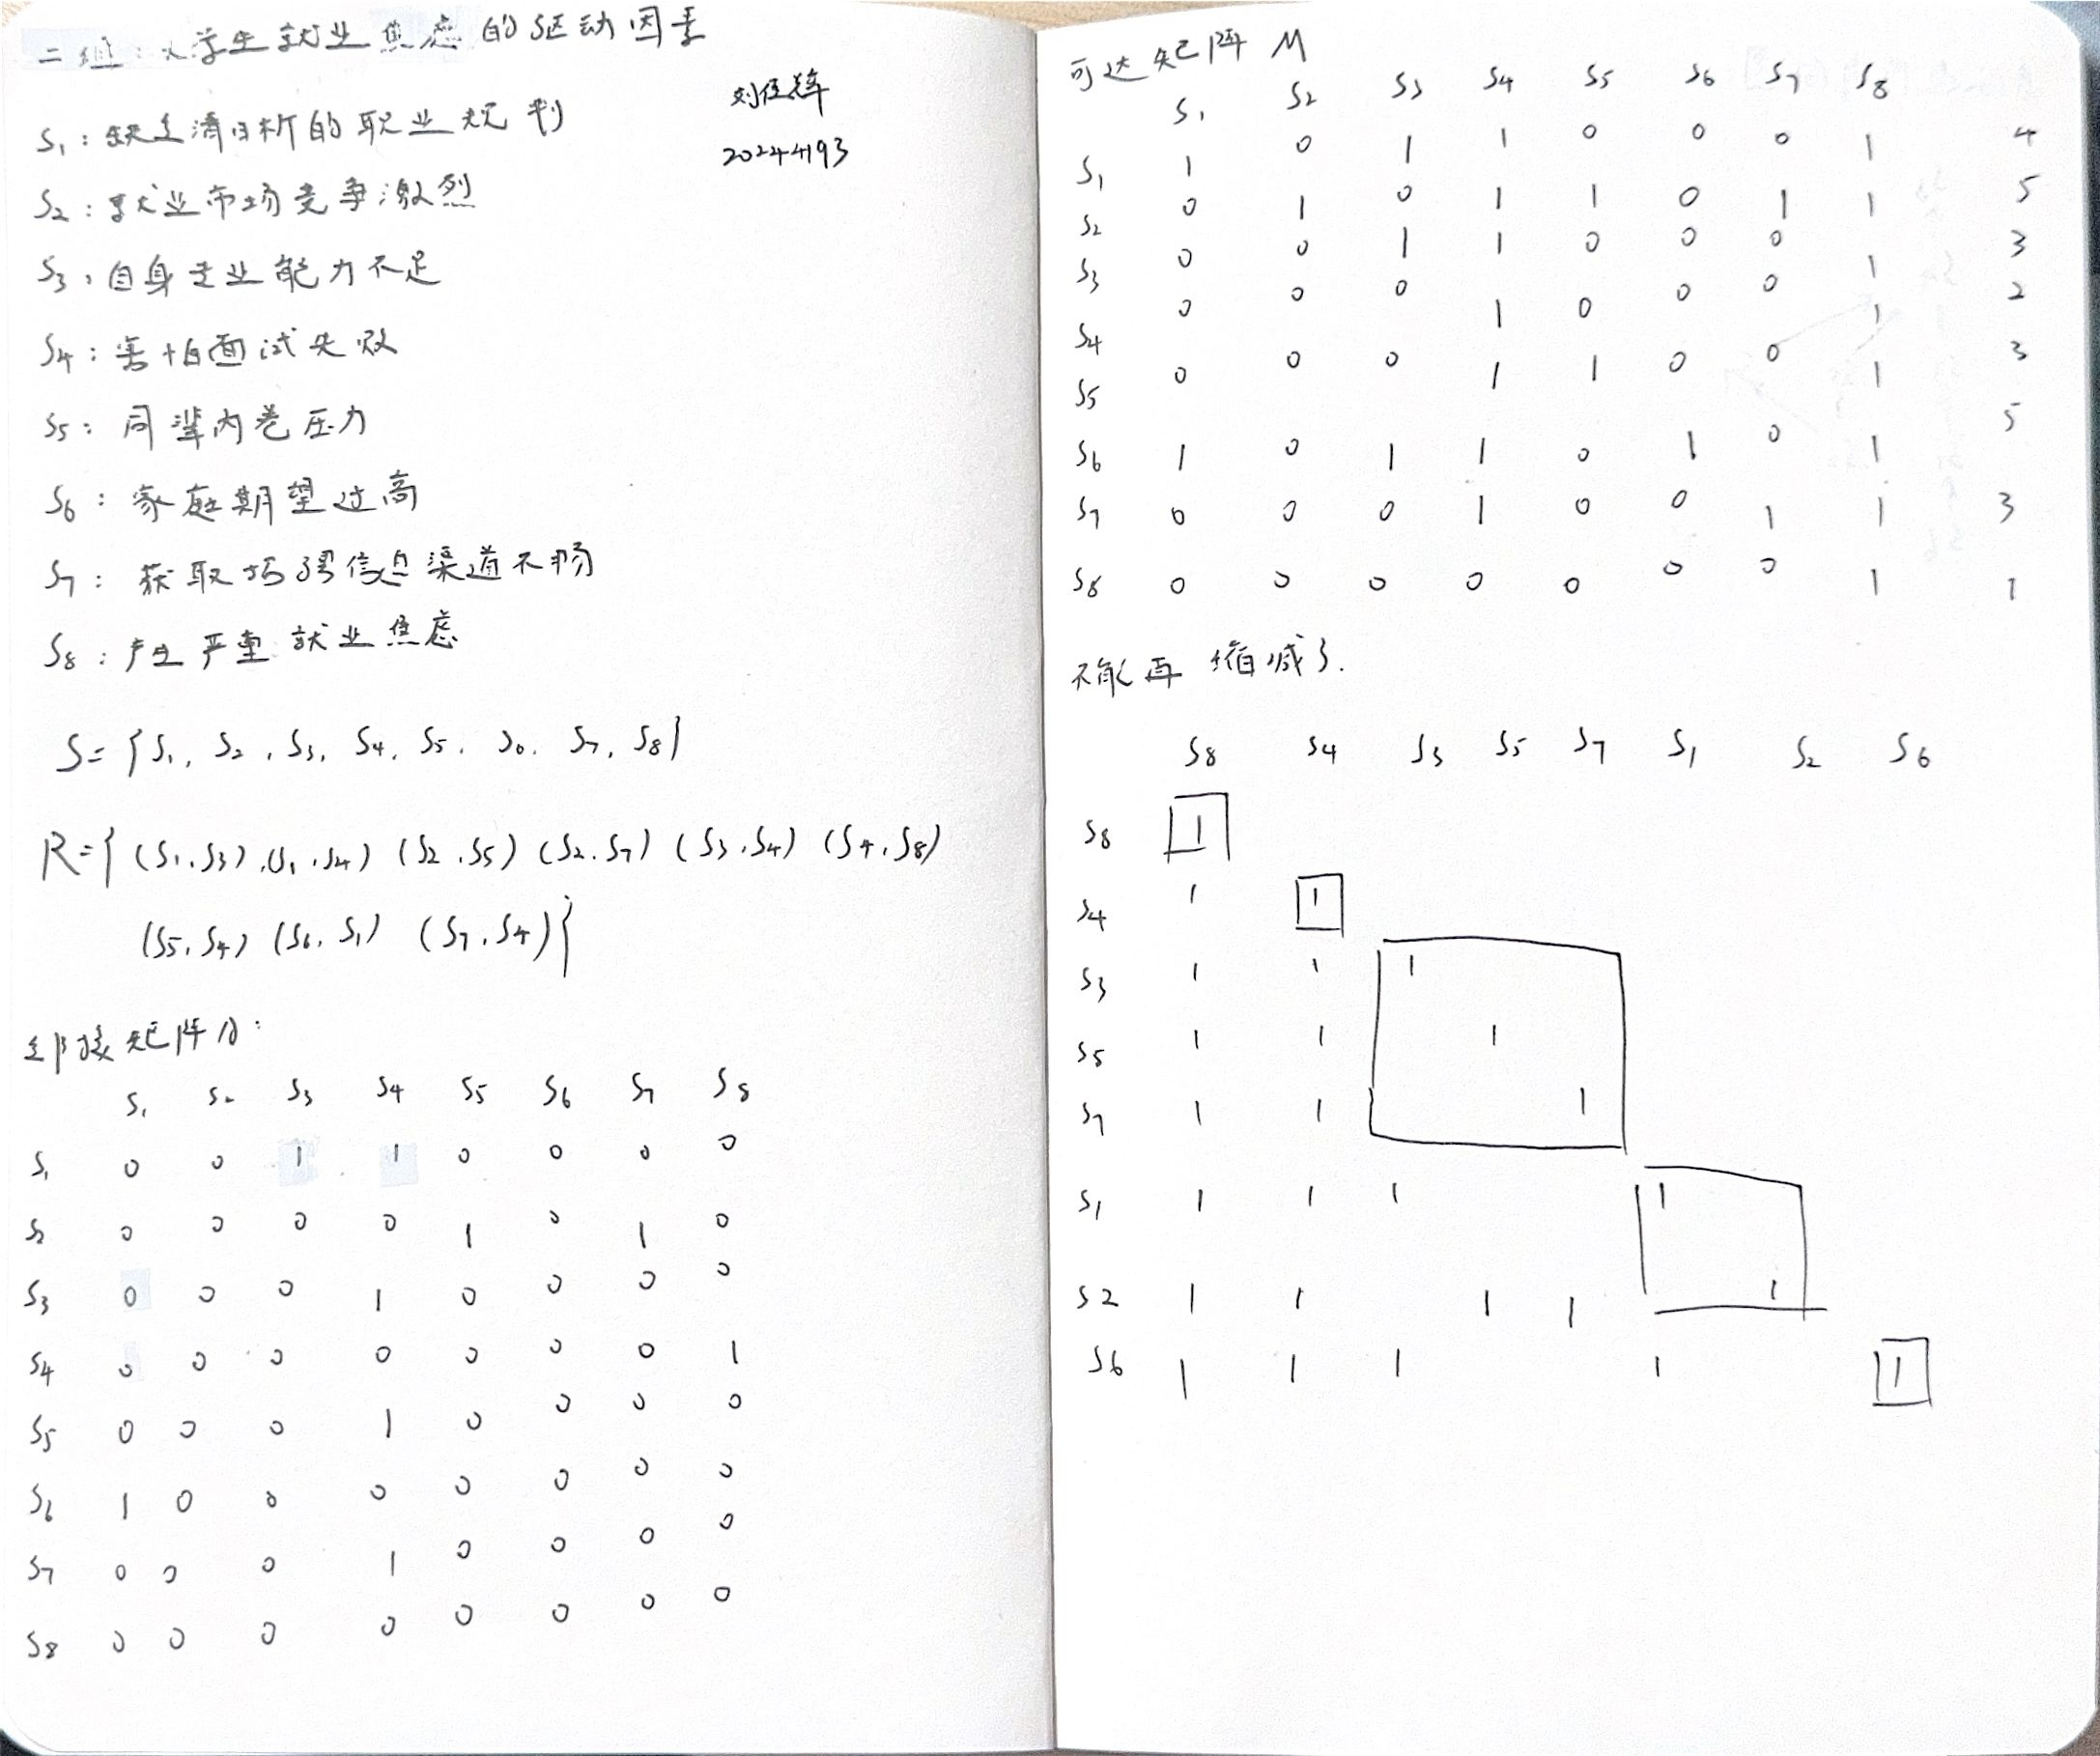
\includegraphics[width=\textwidth,height=0.82\textheight,keepaspectratio]{1.jpg}
  \caption{手算草稿（一）}
  \label{fig:handwritten-1}
\end{figure}

\begin{figure}[H]
  \centering
  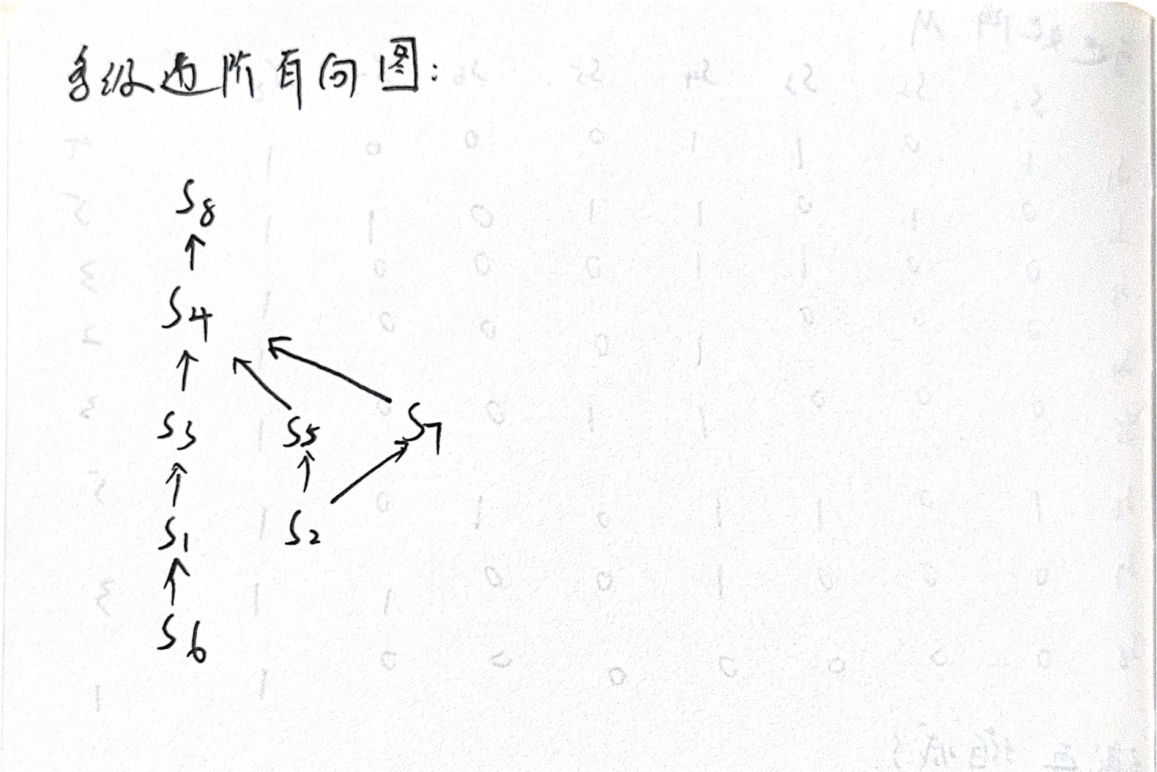
\includegraphics[width=0.7\textwidth,height=0.82\textheight,keepaspectratio]{2.jpg}
  \caption{手算草稿（二）}
  \label{fig:handwritten-2}
\end{figure}

\end{document}